\subsection{Counter Examples for Programs with Conditionals}
    
        In addition to the above proof, we also show certain counter examples where reordering may not be safe to do. This faciliates better understanding of the proof and its arguments. These counter examples are with respect to reordering of writes. 

     

        The example below shows a case with a conditonal having two branches where reordering $e$ and $d$ is not safe. 
        \begin{figure}[H]
            \centering 
            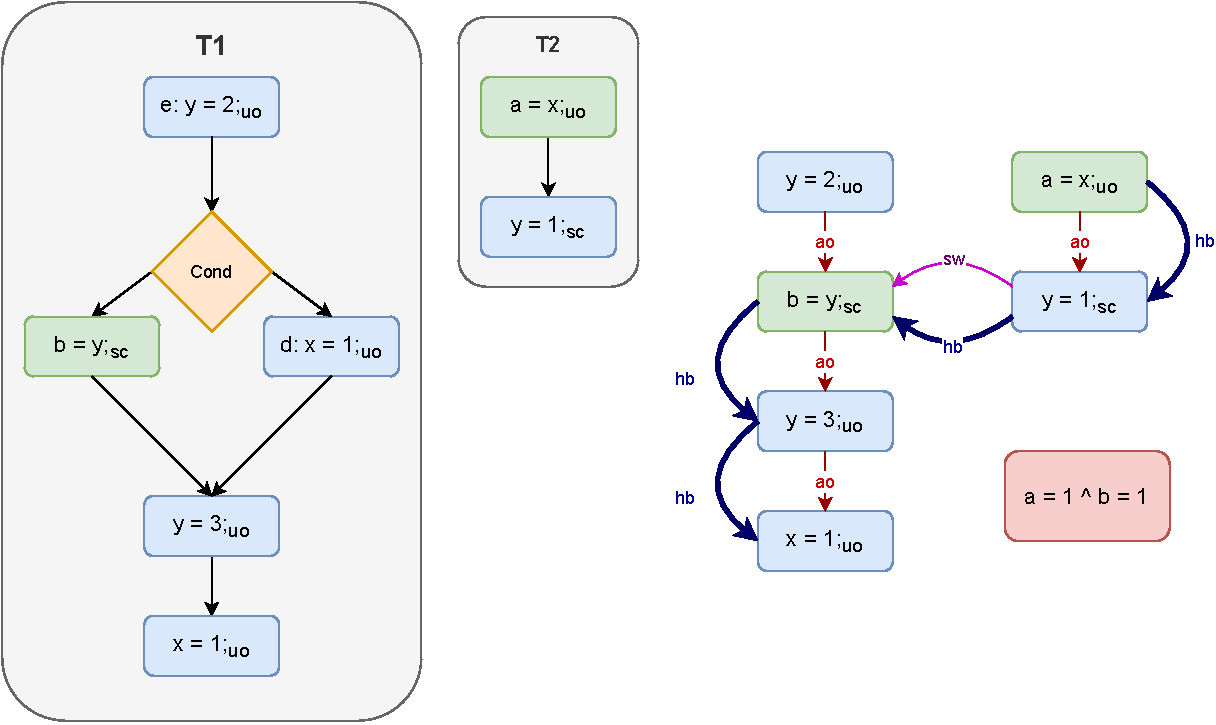
\includegraphics[scale=0.7]{5.InstructionReordering/5.ValidReorderingProgram/CounterExamples1a(Conditionals).pdf}
            \caption{}
        \end{figure}
        The figure on the left above shows an example of such a program.  
        The figure on the right shows the Candidate Execution where the red box outcome is not allowed when the left branch of the conditional is taken.
        \begin{itemize}
            \item From the Candidate Execution, we can infer $\reln{\{a=x;_{uo}\}}{hb}{\reln{\{y=1;_{sc}\}}{hb}{\reln{\{b=y;_{sc}\}}{hb}{\reln{\{y=3;_{uo}\}}{hb}{\{x=1;_{uo}\}}}}}$.
            \item By Axiom \ref{CoRe}, the read $a$ cannot have value of $x$ read as $1$. 
            \item This inference was due to $\reln{\{a=x;_{uo}\}}{hb}{\{x=1;_{uo}\}}$.
        \end{itemize}

        \begin{figure}[H]
            \centering 
            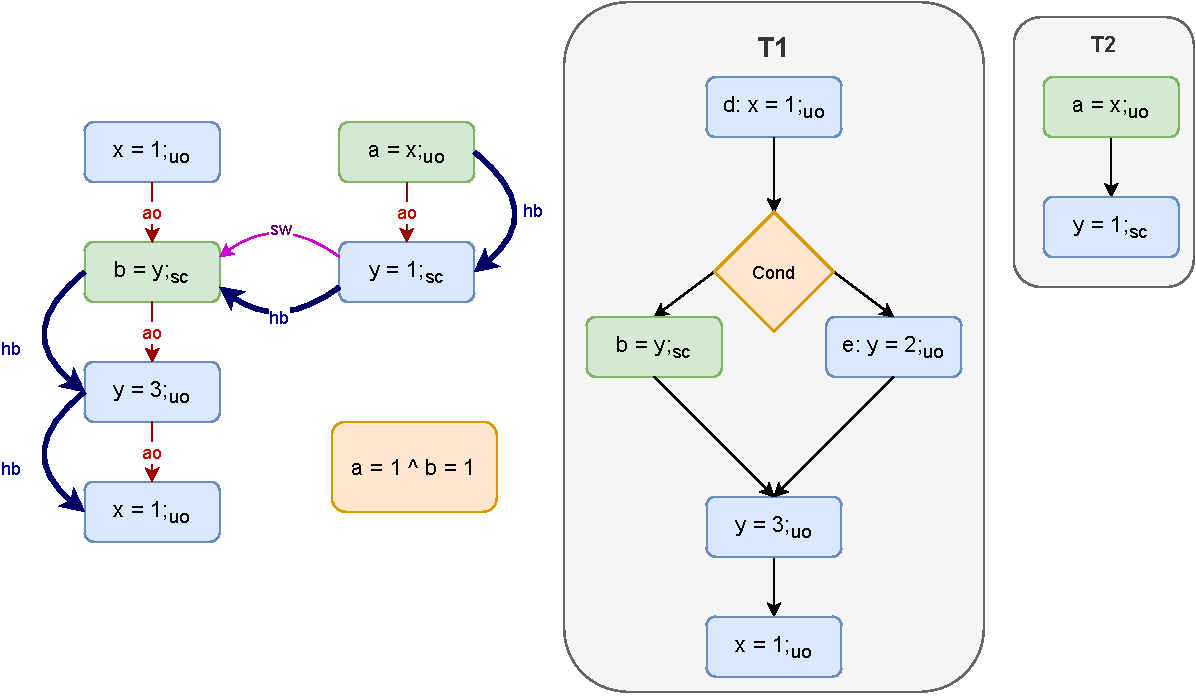
\includegraphics[scale=0.7]{5.InstructionReordering/5.ValidReorderingProgram/CounterExamples1b(Conditionals).pdf}
            \caption{}
        \end{figure}
        The figure on the right above shows the program after reordering $e$ and $d$.  
        The figure on the left shows a Candidate Execution where the yellow box outcome is allowed when the left branch of the conditional is taken\footnotemark.

        \footnotetext{Notice that the above counterexample can also be attributed to introducing a new write $x=1$ in a candidate.}

        \begin{itemize}
            \item From the Candidate Execution, we can infer $\reln{\{a=x;_{uo}\}}{hb}{\{x=1;_{uo}\}}$. 
            \item But there is no $\stck{_{hb}}$ relation with event $d$ and the read to $x$, i.e. $\neg \reln{\{a=x;_{uo}\}}{hb}{d:\{x=1;_{uo}\}}$
            \item No Axiom restricts the read $a$ to have value of $x$ as $1$.
        \end{itemize}

        The example below is a counter example where the conditional has only one branch.

        \begin{figure}[H]
            \centering 
            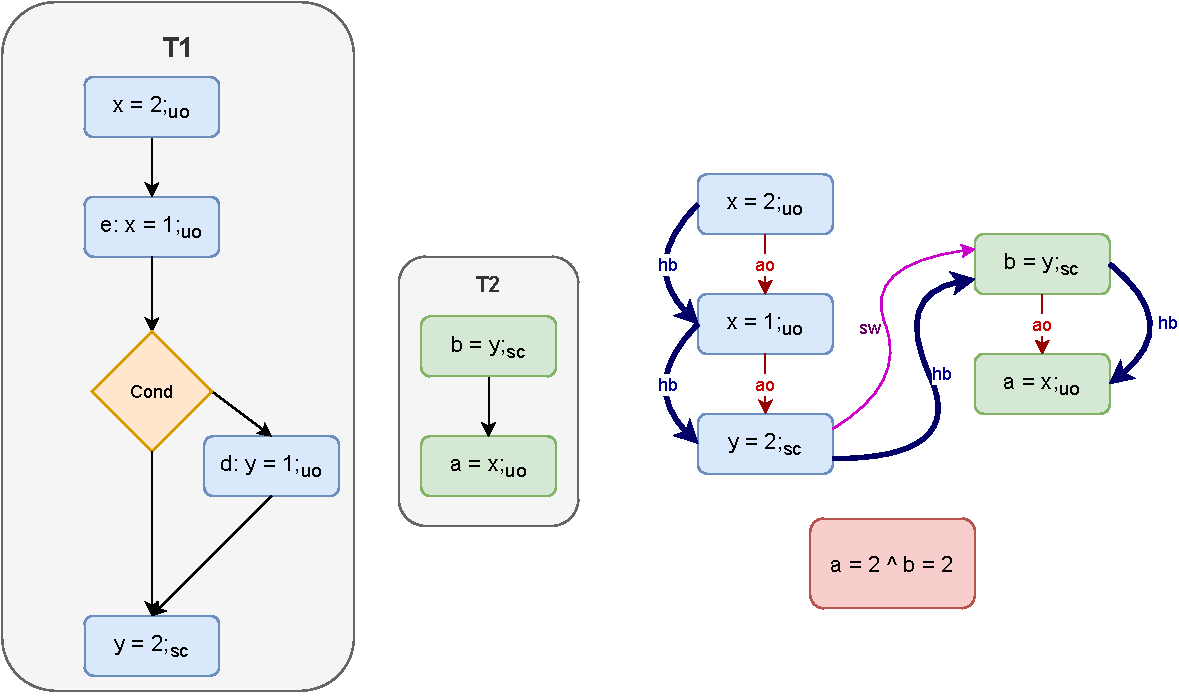
\includegraphics[scale=0.7]{5.InstructionReordering/5.ValidReorderingProgram/CounterExamples2a(Conditionals).pdf}
            \caption{}
        \end{figure}
        The figure on the left above shows an example of such a program.  
        The figure on the right shows the Candidate Execution where the red box outcome is not allowed when the conditional branch is not taken.
        \begin{itemize}
            \item From the Candidate Execution, we can infer $\reln{\{x=2;_{uo}\}}{hb}{\reln{\{x=1;_{uo}\}}{hb}{\reln{\{y=2;_{sc}\}}{hb}{\reln{\{b=y;_{sc}\}}{hb}{\{a=x;_{uo}\}}}}}$.
            \item By Axiom \ref{CoRe}, the read $a$ cannot have the value of $x$ to be read as $2$.  
            \item This inference was due to the realtion $\reln{\{x=2;_{uo}\}}{hb}{\reln{\{x=1;_{uo}\}}{hb}{\{a=x;_{uo}\}}}$.
        \end{itemize}

        \begin{figure}[H]
            \centering 
            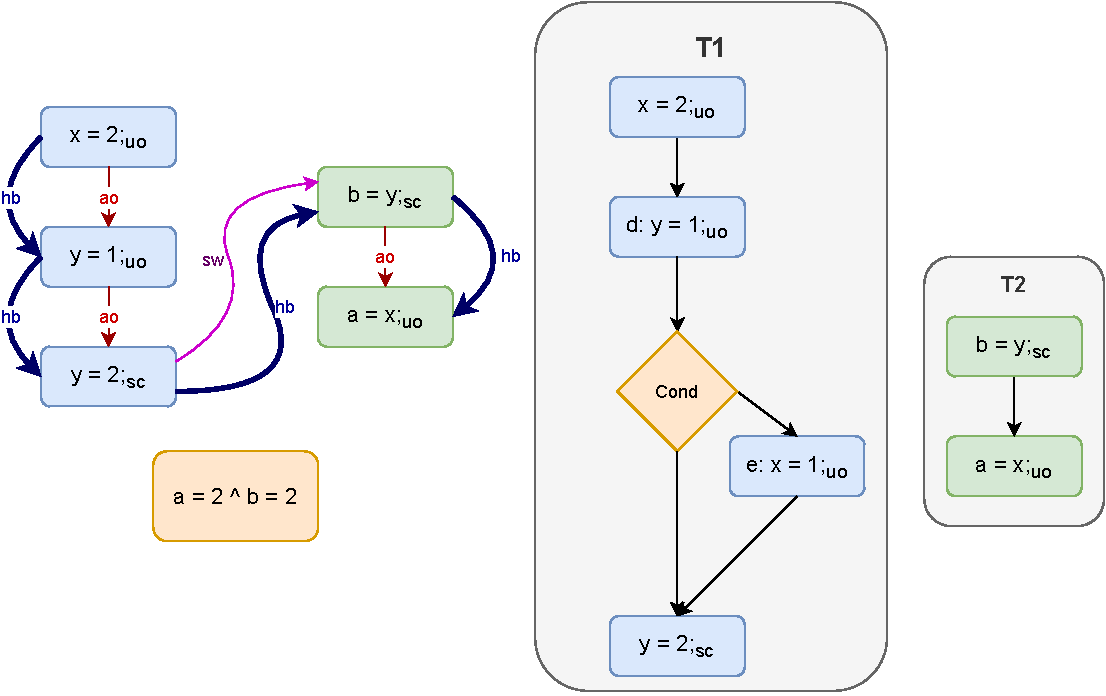
\includegraphics[scale=0.7]{5.InstructionReordering/5.ValidReorderingProgram/CounterExamples2b(Conditionals).pdf}
            \caption{}
        \end{figure}
        The figure on the right above shows the program after reordering $e$ and $d$.  
        The figure on the left shows a Candidate Execution where the yellow box outcome is allowed when the conditional branch is not taken\footnotemark.
        
        \footnotetext{Notice that the above counterexample can also be attributed to the elimination of a write $x=1$.}

        \begin{itemize}
            \item From the Candidate Execution, we can infer $\reln{x=1;_{uo}}{hb}{a=x;_{uo}}$. 
            \item But there is no $\stck{_{hb}}$ relation with event $e$ and the read to $x$, i.e. $\neg \reln{e:x=1;_{uo}}{hb}{a=x;_{uo}}$.
            \item No Axiom restricts the read $a$ to have value of $x$ as $2$.
        \end{itemize}

%-----------------------------------------------------------------------------------------------------------------------------------
    We leave the rest of the cases as an exercise to the avid reader\footnotemark.

    \footnotetext{While showing reordering of reads, one must note that the introduction of new observable behaviors is dependant on the fact that a candidate execution has a local variable which must have not been there beacause the conditional branch was not taken. Note that this fact does not rely on the consistency rules of the memory model. It could be the case that the compiler instantiates the local variables to some default value (say 0), and then decides to reorder a read outside a conditional on the assertion that the read of local variable will return the same constant value. Having such an assertion in general might not be always certain.}
%------------------------------------------------------------------------------------------------------------------------------------------